\chapter[Introduction]{Introduction}
\label{chap:intro}

% Leave space between title and quote or publication note.  This has often been
% 10cm for a quote and 8 cm for a reference, but this is really up to you.
%\vspace{8cm}

%\vfil\eject\clearpage
\clearpage It has long been known that stars in the solar neighborhood
have vertical scale-heights and velocity dispersions that increase
with age \citep[e.g.,][]{Wielen74}. This phenomenon is referred to as
``disk heating'', and the origin of this heating process has never
been settled. Unfortunately, our empirical constraints on disk heating
come only from the solar cylinder in the Milky Way and a few crude
measurements of low-mass edge-on spirals close enough for HST
star-counts \citep{Seth05a}. This scant data is insufficient to
resolve several outstanding questions: How does the heating rate
evolve with time and radius?  Why does disk heating in the Milky Way
appear to saturate after about 5 Gyr?  What, then, gives rise to the
thick disk?  And is heating in the Milky Way representative of disk
galaxies in general? Answers to these questions have critical
implications for our picture of disk evolution, all the more poignant
given recent observational claims that high-redshift ionized gas disks
are dynamically hot, clumpy, and thick \citep{Forster-Schreiber09} and
models \citep{Bird13} that predict the formation of observed current
disk structure from these high-redshift disks.

Clearly more data is needed, and the rise of resolved spectroscopic
surveys of external galaxies (e.g., MaNGA, SAMI, CALIFA) will offer a
new window into the distribution of stellar populations outside the
Milky Way. However, these surveys lack the spatial resolution
necessary to make detailed comparisons to the substructures seen in
the Milky Way and it is crucial to complement their broad scope with
focused measurements of nearby galaxies. NGC 891 offers an attractive
target for such a study; it is nearby, almost perfectly edge-on, and
is thought to be a good Milky Way analog. In this thesis I present a
study of stellar populations in NGC 891, specifically where these
populations fall in a six dimensional space containing three position
dimensions along with age, metallicity, and extinction.

The rest of this chapter is organized as follows: in
\S\ref{intro:sec:MW} I review the picture of disk formation as
revealed locally in the Milky Way; in \S\ref{intro:sec:SSP} I discuss
the details of the methods (namely full-spectral fitting) that will be
used to measure populations in NGC 891; and in \S\ref{intro:sec:fiber}
I give a brief overview of fiber integral field units (IFU) and lay
the groundwork for the introduction of HexPak/\GP; the world's first
dual-head, variable-pitch IFU.

\section{Stellar Populations in the Milky Way}
\label{intro:sec:MW}
\begin{figure}
  \centering
  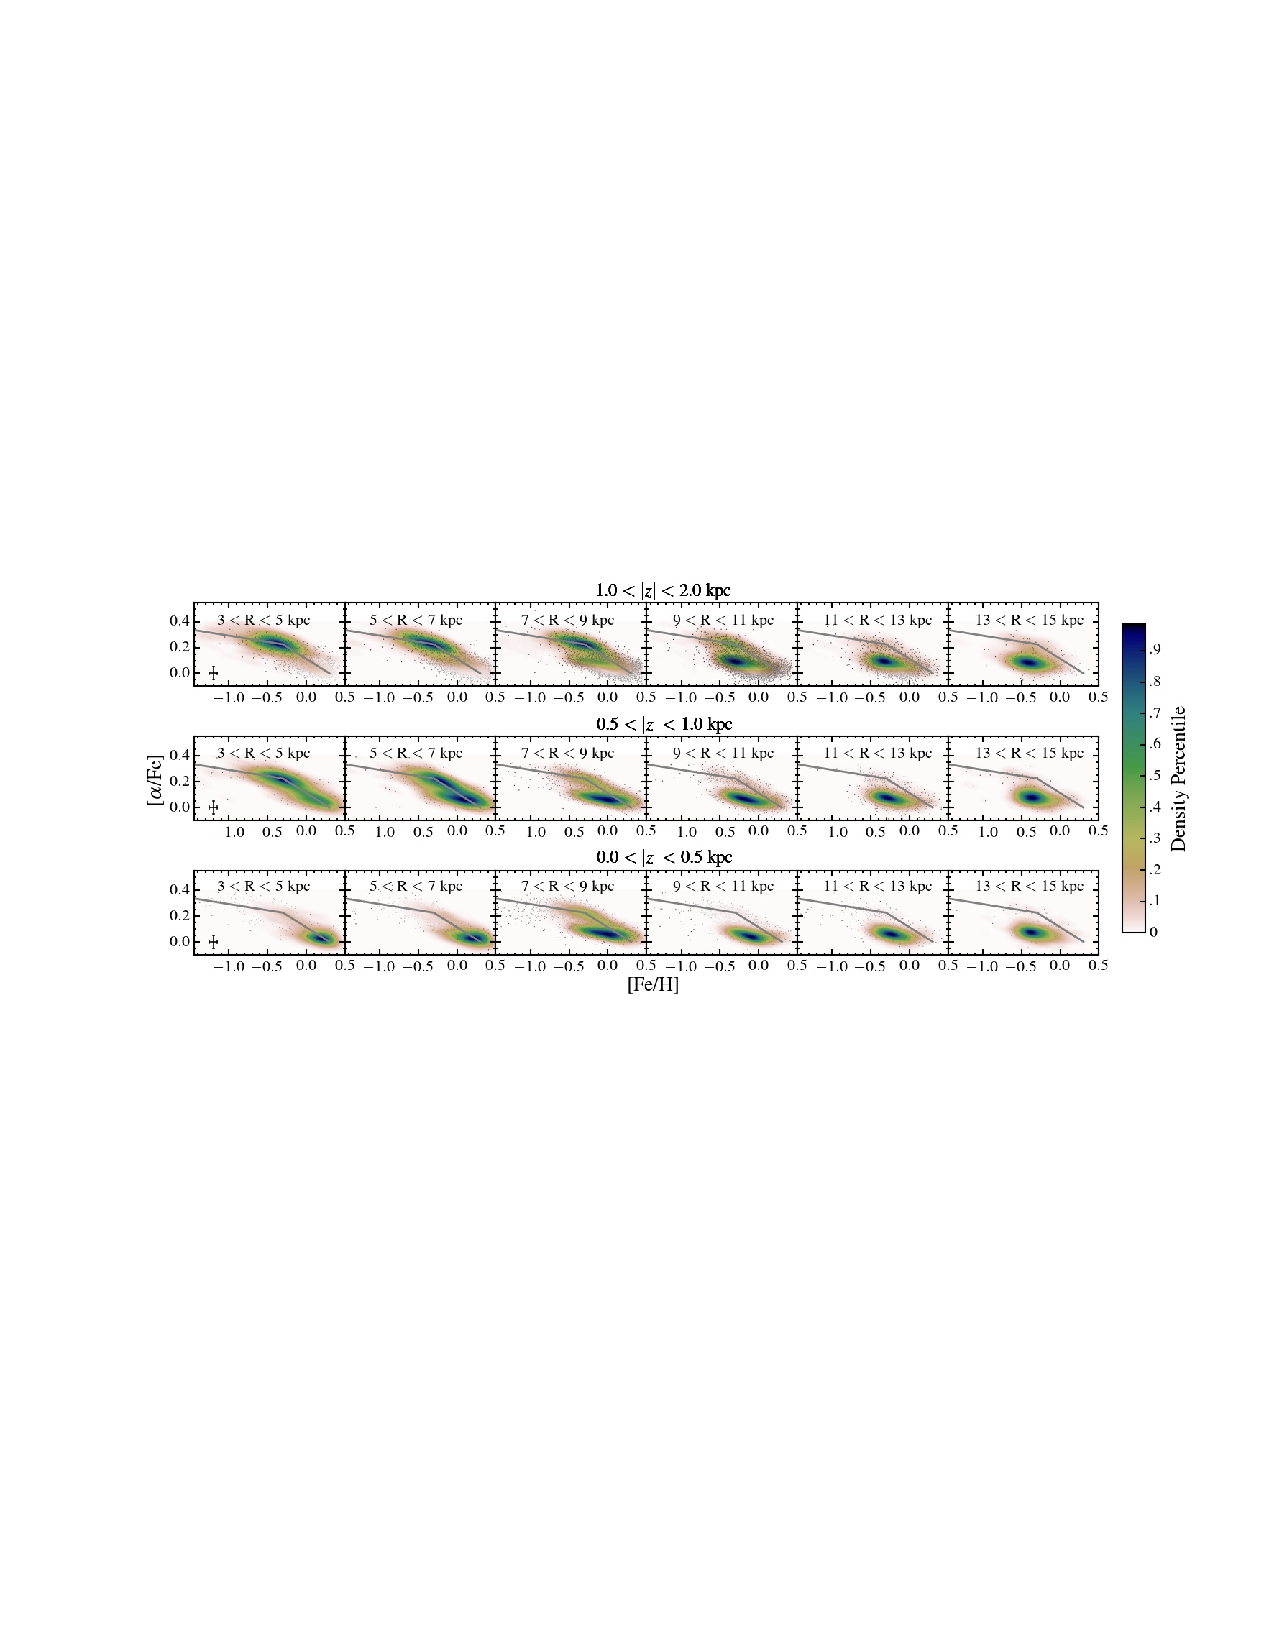
\includegraphics[width=\textwidth]{Introduction/figs/hayden_15.pdf}
  \caption[Metallicity and abundance of solar cylinder stars as a
  function of radius and
  height]{\fixspacing\label{intro:fig:hayden}The distribution of stars
    near the Sun in the [$\alpha$/Fe] vs. [Fe/H] plane, presented in a
    grid of radius and height. From \citet{Hayden15}.}
\end{figure}

By the middle of the last century it was well established that the
scale-heights and velocity dispersions of stars in the solar
neighborhood increase with age \citep[see][for a summary of this early
work, particularly the chapters contributed by Elvius and
Delhaye]{Blaauw65}. The seminal work by \citet{Roman50} demonstrated
that the disk kinematics also depended on metallicity.  Today these
patterns are known in the literature on Galactic archaeology as
age-velocity-metallicity (abundance) relations \citep[AVM$\alpha$-R;
e.g.,][]{Aumer09,Minchev14}. Observational advances continued for the
solar neighborhood \citep[e.g.,][]{Edvardsson93, Dehnen98,
  Nordstrom04}, and by the beginning of this century the complexity of
these relations had been mapped throughout much of Milky Way (MW) by
wide-field spectroscopic surveys (e.g., RAVE, \citealt{steinmetz06a};
BRAVA, \citealt{howard08a}, SEGUE, \citealt{yanny09a}, LAMOST,
\citealt{zhao12a} GALAH, \citealt{desilva15a},
Gaia-ESO,\citealt{gilmore12a}; and APOGEE-1 and -2,
\citealt{Majewski15}). The radial gradients in these relations are
beautifully shown in Figure \ref{intro:fig:hayden} (from
\citet{Hayden15}), illustrating the usefulness of both metallicity and
abundance as well-known, complementary chemical-evolutionary
tracers. Despite a century of remarkable progress, two broad but
intertwined questions remain: (i) What are the astrophysical processes
(i.e., the chemo-dynamical explanation) leading to the observed
relations?; and (ii) are these patterns generic for spiral disks or
specific to the Milky Way?

\begin{figure}
  \centering
  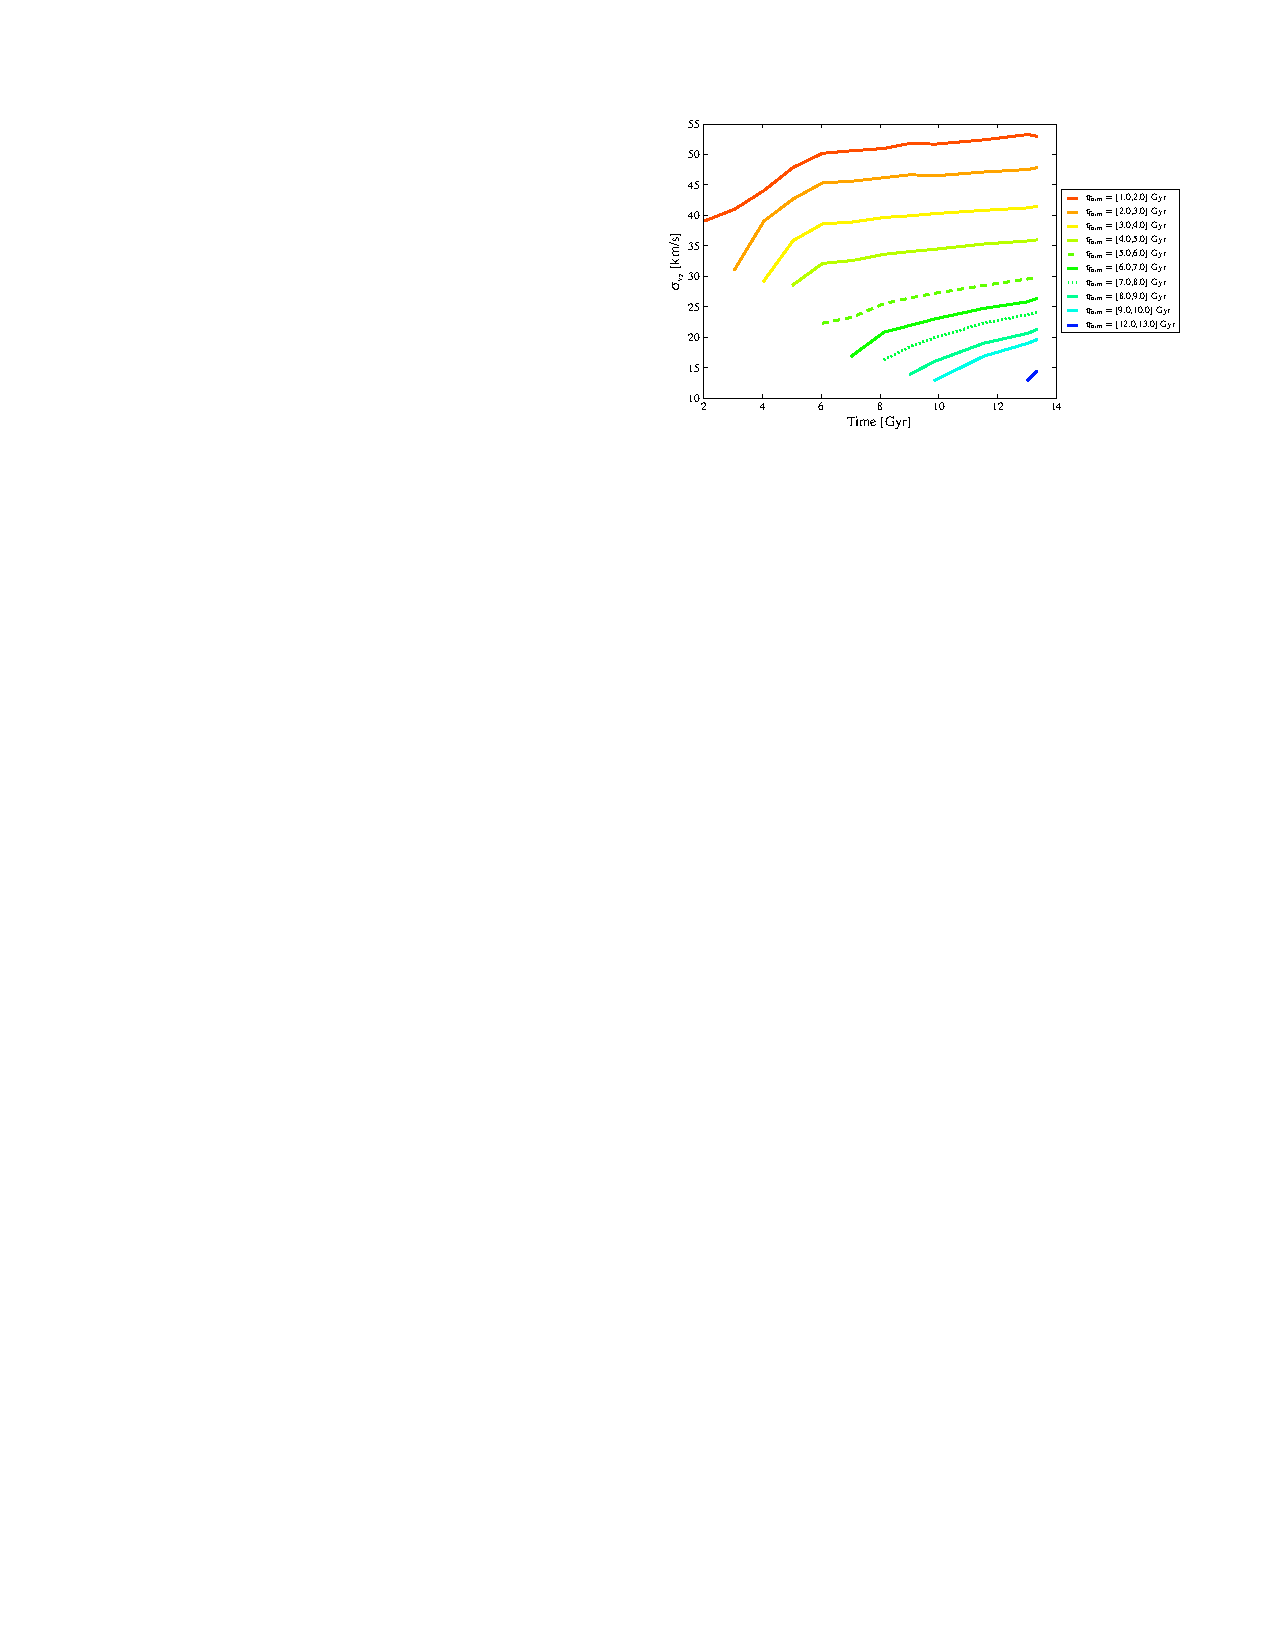
\includegraphics[width=0.8\textwidth]{Introduction/figs/bird_13.pdf}
  \caption[Dynamical settling in a Milky-Way-like galaxy
  model]{\fixspacing\label{intro:fig:bird}Vertical velocity dispersion
    of stellar populations with different formation ages as a function
    of time. These models are based on hydrodynamical simulations of a
    Milky-Way-like disk galaxy. From \citet{Bird13}}
\end{figure}

Setting aside chemical evolution for simplicity, there has been a
long-standing debate about the origin of the vertical stratification
of disk stars in phase-space as a function of age. This stratification
is known as the the age-velocity relation, or AV-R. Historically the
argument has been in the context of dynamical heating from two-body
scattering \citep{Spitzer51}, but the source of this scattering has
been debated \citep[e.g., giant molecular clouds, transient spiral
structure, or dwarf satellite
galaxies][]{Spitzer51,Spitzer53,Wielen77,Quinn93,Binney00}, and none
have proven satisfactory to explain the MW's thick disk.  This
framework has been salvaged but also up-ended by relatively recent
evidence for the increasing turbulence (and presumably thickness) of
ionized gas in disks at higher redshifts
\citep{Weiner06,Forster-Schreiber09,Wisnioski15}. It seems plausible
that early phases of disk formation involved gas cooling, leaving
behind an old, thick-disk stellar component
\citep{Brook04,Bournaud09}. However, thinner relic layers would also
emerge as time progressed \citep{Bird13}, depending critically on the
cooling time-scale for the gas in the presence of star-formation, AGN
feedback, and accretion. Figure \ref{intro:fig:bird} shows an example
of this theory; vertical velocity dispersion does slightly increase as
stars age (i.e. ``heating''), but the dominant trend is that more
recently formed populations are dynamically cooler. Ironically, this
``settling'' of the stellar disk is not unlike the predictions of
monolithic collapse from \citet{ELS}, albeit now consistent in the
context of bottom-up, or hierarchical structure formation as seen in
recent simulations \citep[e.g.,][]{Bird13,Martig14a}.  It is no longer
clear if, loosely speaking, disks ``heat'' or ``cool'' to form the the
vertical stratification of disk stars in phase-space, and likely both
modes play a role at late and early times, respectively. For this
reason we refer instead to ``dynamical stratification'' as a
phenomenon that captures both general physical processes.

The recent simulations noted above show there is a rich history of
radial and vertical build up of stellar populations that involves an
interplay between the cooling of the gas, the impact of mergers and
accretion, and, at late times, the classical heating processes noted
above.  This richness suggests the possibility for a diversity of
astrophysical paths in disk formation that could lead to significantly
different structure in galaxies, exhibited in their
AVM$\alpha$-Rs. Hence, the broader question of whether the MW is
representative of the external disk galaxy population becomes salient.

%% Maybe move to previous section
Little is known about the dynamical stratification rates for stars in
spiral galaxies outside the Milky Way, but recent studies of stellar
populations and dynamical stratification in low-mass spiral galaxies
\citep{Seth05a,Bernard15} have shown dramatic differences in the
age-metallicty and age-velocity dispersion relations when compared to
the Milky Way. Recent measurements of the stellar velocity dispersions
in M31 \citep{Dorman15} show that there are gradients in dispersion
with age and metallicity, but with amplitudes and time-scales that are
larger than in the MW. Differences in velocity dispersion amplitudes
may reflect a more massive or thinner M31 disk, but possibly also a
different dynamical history -- for gas settling or stellar dynamical
heating. Clearly more data on the stellar properties of external
galaxies is needed. The above studies serve as a gold standard since
they are based on studies of resolved stellar populations. Because
there are no massive spiral galaxies outside of the Local Group for
which we can resolve stellar populations at surface-densities high
enough to probe most of the disk, it is imperative to undertake
studies based on integrated starlight.

\section{Deriving Population Properties with Full Spectrum Fitting}
\label{intro:sec:SSP}
\begin{figure}
  \centering
  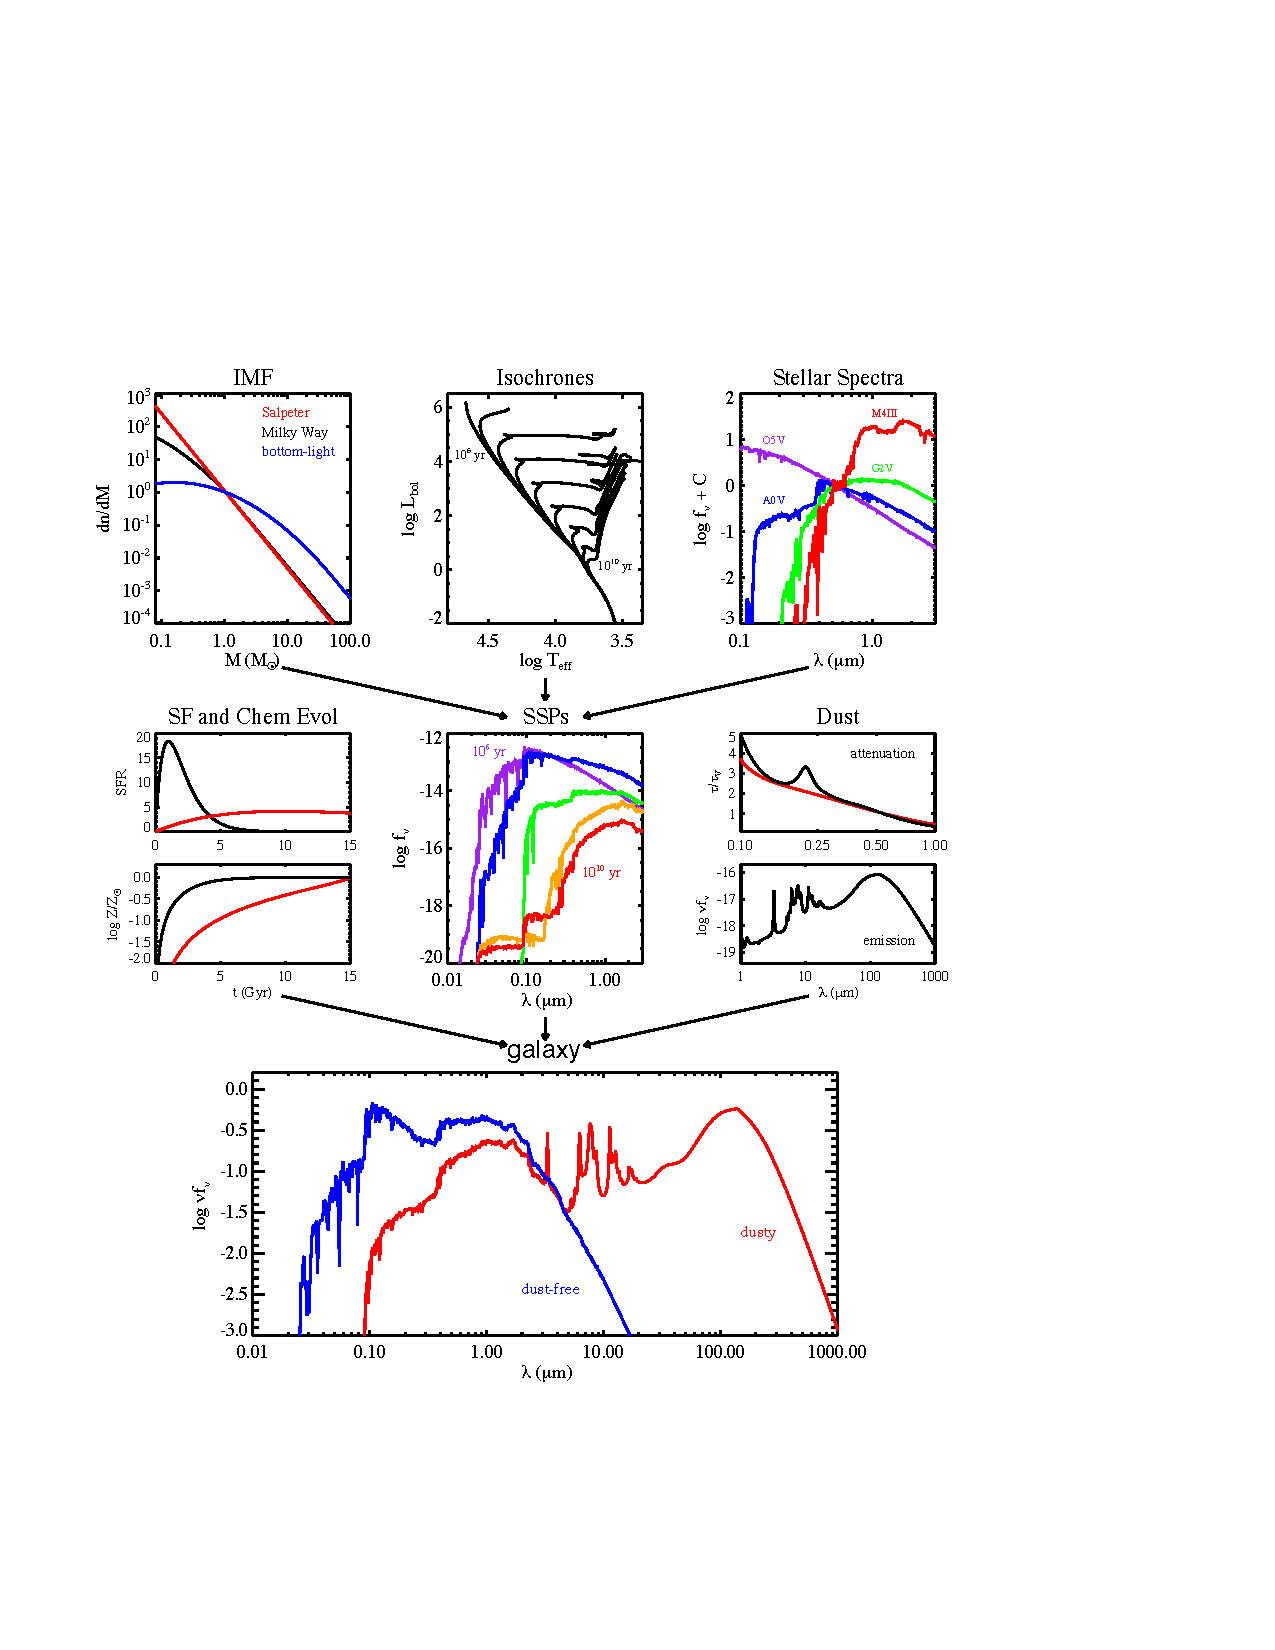
\includegraphics[width=0.8\textwidth]{Introduction/figs/conroy_13.pdf}
  \caption[Schematic of full spectrum
  fitting]{\fixspacing\label{intro:fig:conroy}The important components
    of full spectrum fitting. An initial mass function (IMF),
    isochrones, and spectra are combined to construct individual
    SSPs. Multiple SSPs are then combined, with and assumed star
    formation history and dust properties, to form a model
    galaxy. From \citet{Conroy13}.}
\end{figure}

In this work we employ full-spectral fitting to measure age,
metallicity, and extinction as a function of radius and height in NGC
891. The idea of modeling integrated starlight (i.e., a spectrum) to
measure galaxies properties has a long history since \citet{Spinrad71}
first manually mixed stars together, and modern techniques employ a
variety of sophisticated methods to extract the maximum about of data
from each wavelength. Regardless of the specific method, all attempts
at full-spectrum fitting require the same basic ingredients: (i) a
library of stellar spectra, whether empirical or synthetic, (ii) a set
of isochrones that encapsulate how stars evolve with time, and (iii)
an initial mass function (IMF). With these three components
Astronomers can construct simple stellar populations (SSPs); a set of
stars of the same age and same metallicity/abundance with a mass
distribution determined by the IMF. To simulate an entire galaxy
multiple SSPs of different ages and metallicities are combine together
to produce a complex stellar population (CSP), which requires assuming
both a star formation history (SFH) and the distribution/properties of
dust in the galaxy. An excellent discussion of this process can be
found in \citet[and his diagram shown in Figure
  \ref{intro:fig:conroy}]{Conroy13}.

Within the general picture painted above there exists a wide range of
options and data. It is common for SSP libraries to be constructed
with the Padova isochrones \citep{Bertelli94, Girardi00, Marigo08}
because these models cover the widest range of stellar age and
chemical compositions, but other models are often used for their focus
on specific epochs of stellar evolution. For example high-mass stars
(Geneva \citep{Schaller92,Meynet00}), low-mass stars ($Y^2$
\citep{Yi01,Yi03}, or Dartmouth \citep{Dotter08}), and even very
low-mass stars (Lyon \citep{Chabrier97,Baraffe98}). In this work we
use exclusively the Padova isochrones because our observations, by
their very nature, are light-weighted and therefore the specific
details of low mass stars are relatively unimportant.

The choice of IMF can also affect the final modeled galaxy
spectrum. The canonical IMF of \citet{Salpeter55} was based on
observations of the Solar Cylinder in the Milky Way, and there is so
far little evidence that the IMF is appreciably different elsewhere in
the Universe \citep{Bastian10}. More recent observations have refined
the specific form of the IMF \citep{Kroupa01, Chabrier03}, but the
general picture remains the same. We use the IMF of \citet{Chabrier03}
because it is physically motivated and provides a good fit to low-mass
and brown dwarf star counts in the Milky Way
\citep{Bruzual03,Chabrier01,Chabrier03}.

Finally, the construction of SSPs depends on the stellar library
used. In this work we consider only empirical stellar libraries, and
more specifically the STELIB \citep{LeBorgne03} and MILES
\citep{Sanchez-Blazquez06} libraries. The main strength of empirical
libraries is that they get the chemistry right by default, as indeed
they must. The cost of this accuracy, however, is a very limit
sampling of the entire parameter space of stellar evolution. For
example, as is discussed in \S\ref{891_2:sec:ma11}, the MILES library
very coarsely samples the metallicty/age plane and doesn't have any
spectra for ages below \val{6.5}{Myr}. 
% Ultimately, we use the STELIB
% library because it more finely samples stars of different ages, but
% warn that it still lacks a detailed view of how spectra change with
% metallicity.
As discussed in \S\ref{891_2:sec:SSP_sets} we ultimately use the SSPs
of \citet{Bruzual03}, which are constructed with the Padova
isochrones, Chabrier IMF, and STELIB library. We note, however, that
over the wavelength range we consider ($\val{3800}{\AA}
\leq\lambda\leq \val{6800}{\AA}$) the differences in spectral shape
caused by different assumptions/models are minimal.

More directly relevant to our work is the assumption about the SFH
that is used to construct galaxies (CSPs) from SSPs. A common choice
for SFH is the so called $\tau$-model where the star formation rate
(SFR) follows an exponential function with a single scale parameter,
$\tau_\mathrm{SF}$. This analytic form is based on closed-box models
where the SFR depends linearly on gas density \citep{Schmidt59} and
offers an attractive, one parameter, parameterization of the SFH. In
this work we chose to use a non-parametric SFH (as discussed in
\S\ref{891_2:sec:SSP_method}) which allows us to reduce the
systematics in our results that arise from forcing an analytic form of
the SFR (systematics are not completely eliminated, however, as
discussed in \S\ref{891_2:sec:sys_err}). Using this method results in
a much larger set of free parameters and puts more strain on the
fitting code, but our data have high enough signal to noise
(\val{\asim 30}{px^{-1}}) to make it a viable option.

Once model galaxies are constructed there are a multitude of methods
available to fit them to our data, for example those of
\citep{Cappellari04, Tojeiro07,Chen12, CidFernandes05, Ocvirk06,
  Wilkinson15, Sanchez16}. Regardless of the method used these fits
face the same common issues; namely how to deal with known
degeneracies between age, metallicity, and extinction
\citep{Oconnel76,Aaronson78,Worthey94,dePaz02}. In some methods the
extinction degeneracy can be mitigated by removing the overall
continuum from both the data and models before fitting
\citep[e.g.,][]{Ocvirk06,Wilkinson15} and then recovering an
extinction estimate either by measurements of gas emission (i.e., the
Balmer decrement) or separate analysis of the ``best fit'' galaxy
spectrum. Metallicity and age are more closely entwined and the
degeneracy between them more difficult to break. In this work we
attempt to quantify the uncertainties that arise from similarities
between SSPs that are degenerate with age and metallicity (see
\S\ref{sec:fit_err}), but note that we have not addressed systematic
uncertainties that may arise from our choice of model SSPs.

\section{A Fiber Optic Primer}
\label{intro:sec:fiber}
The use of fused silica optical fibers for astronomical observations
was first suggest by \citet{Angel77}, and in the intervening decades
their importance and usefulness to Astronomy has only increased. The
astronomical benefits of fiber optics are essentially two fold:
Firstly, they allow instruments to be decoupled from the telescope
focal plane, which enables the construction of very large and
sensitive spectrographs that are free from the unstable environmental
conditions often found on the observing floor. Secondly, they can be
easily placed at an arbitrary position on the sky while maintaining a
consistent spectrograph input.

A class of fiber optic instruments called integral field units (IFUs)
make great use of this second point. IFUs are a collection of fibers
that are placed in some two-dimensional configuration on the sky and
therefore produce data that exist in three dimensions (two spatial and
one spectral). Some IFUs are designed to efficiently measure the
spectra of a large field of stars, for example HYDRA {\bf REF? Can't
  find it!}, and can have the location of their fibers changed from
program to program. Others have a fiber layout that is fixed and
usually intended for observations of extended objects. SparsePak
\citep{Bershady04,Bershady05} is an excellent example of and IFU of
this type. The trade off for the lack of reconfigurability in fixed
IFUs is a generally tighter fiber packing and therefore improved
spatial coverage.

In the past, difficulties in construction resulted in a cottage
industry of IFU builders, but more recently there has been an
explosion of mass-produced IFUs that have allowed large, resolved
spectrographic surveys like MaNGA \citep{Bundy15}, SAMI
\citep{Croom12}, and CALIFA \citep{Sanchez12} to rapidly expand our
view of the Universe. In this thesis I present \GP and HexPak, a set
of IFUs that are the first in the world to contain fibers of different
sizes, each configured to serve a specific scientific purpose.

\begin{figure}
  \centering
  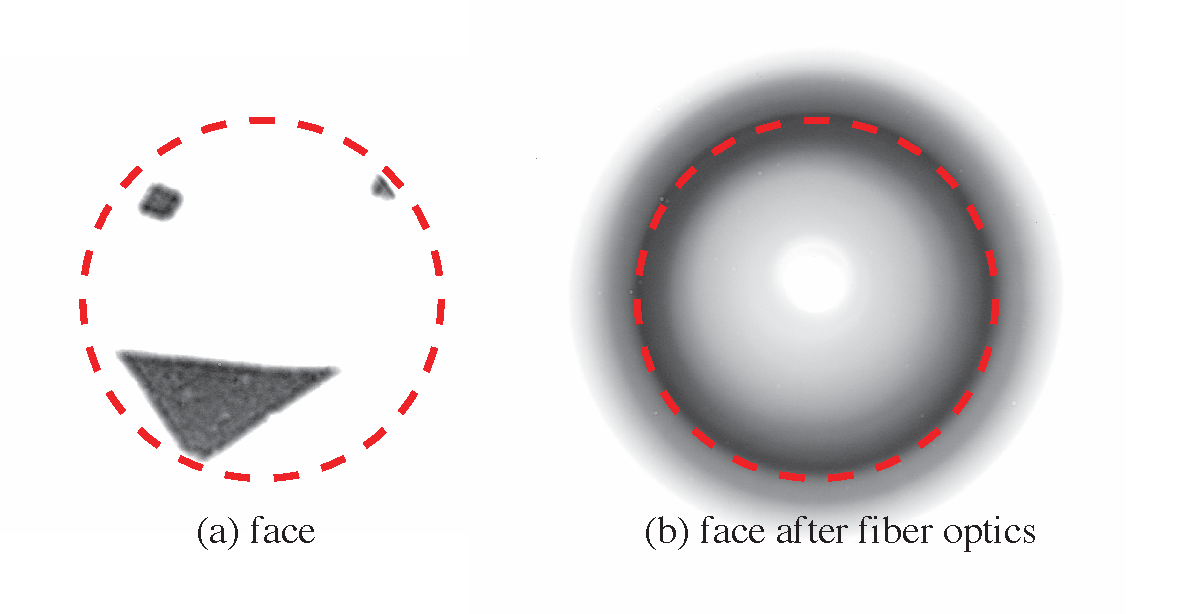
\includegraphics[width=\textwidth]{Introduction/figs/FRDude.pdf}
  \caption[Face on FRD]{\fixspacing\label{intro:fig:FRDude}The effects
    of fiber optics on an input signal. The face in (a) is smeared
    azimuthally and radially during its journey through an optical
    fiber. The red circle corresponds to the same angle at the
    input/output of the fiber.}
\end{figure}

With great power comes great responsibility, however, and fiber optics
affect the light passing through them in ways that have profound
implications for data quality and instrument design. In particular,
fiber optics not only attenuate precious astronomical light, but also
increase the entropy in the beam. The latter effect is referred to as
focal ratio degradation (FRD), whereby light injected into a fiber at
a particular angle emerges from the fiber at a larger angle. An
example of this is seen in Figure \ref{intro:fig:FRDude}; the light
coming out of the fiber (b) has been smeared to angles outside of the
maximum input angle (red circle). This increase in entropy creates a
need for larger (and more expensive) spectrograph optics and can
decrease the total system throughput if not properly accounted for. An
understanding of the causes of FRD can help mitigate its effects and
the first theories placed the blame on microbends along the length of
the fiber \citep{Gloge72,Carrasco94}. Recent studies have suggested
however, that most FRD is caused by scattering at the surface of the
fiber \citep{Avila98,Haynes11,Eigenbrot12}. In the latter scenario it
is likely that surface treatments (i.e., anti-reflective coatings) can
mitigate the effects of FRD.

\clearpage
\phantomsection % Fixes references link in hyperref/PDF index

% Requires thesis.bst to be present (or linked) in chapter subdirectory.
\bibliographystyle{thesis}
\bibliography{Introduction}
